\chapter{Pebble Modeling: Discrete Element Method} \label{modelingDEM}
%%%%%%%%%%%%%%%%%%%%%%%%%%%%%%%%%%%%%%%%%%%%%%%%%%%%%%%%%%%%%%%%%%%%%%%%%%%%%%%%%%%%%%%%%%%%%%
%%%%%%%%%%%%%%%%%%%%%%%%%%%%%%%%%%%%%%%%%%%%%%%%%%%%%%%%%%%%%%%%%%%%%%%%%%%%%%%%%%%%%%%%%%%%%%
This chapter presents the motivations and background of this study. First, it discusses energy usage in our society and the inevitable production of waste mechanical and thermal energies and their ubiquitous nature. This is followed by a brief discussion of common methods of converting ambient mechanical energy and waste heat into useful electrical energy. This chapter concludes with the objectives of this study and the scope of the document.



\section{Background}
\label{sec:dem-intro}



In the framework of the discrete element method, we track particle motion in a Lagrangian sense. In the ensemble of particles, each particle's position, velocity, and acceleration are tracked and updated based on balances (or imbalances) of forces acting upon the particle. The discrete element method for granular material 

\subsection{Numerical Implementation Overview}

The primary computational tools used in this study is LAMMPS (Large-scale Atomic/Molecular Massively Parallel Simulator)\cite{Plimpton1995}; a classical molecular dynamics code. The package of code, maintained by Sandia National Labs (http://lammps.sandia.gov), has many features making it particularly attractive for our use on the simulation of pebble beds. LAMMPS is open-source and written in highly-portable C++ allowing customization of any feature used in modeling. LAMMPS runs with distributed-memory message-passing parallelism (MPI) and provides simple control (manual or automatic) of the spatial-decomposition of simulation domain for parallelizing. The code can be built as a library so that LAMMPS can be coupled to other code or wrapped with Python as an umbrella script. Perhaps most importantly, LAMMPS provides an efficient method for detecting and calculating pair-wise interaction forces; the largest consumer of run-time in the DEM algorithm\cite{Plimpton1995}.

LAMMPS provides modeling of granular particle types; the use of LAMMPS for studying granular material since at least 2001 when Silbert, et al\cite{Silbert2001} studied granular flow on inclined planes. However, usefulness of LAMMPS for studying granular systems was greatly enhanced by LIGGGHTS (LAMMPS Improved for General Granular and Granular Heat Transfer Simulations), a suite of modules included on top of LAMMPS. LIGGGHTS has many academic and industrial contributors from around the world, with the code maintained as open-source by DCS Computing, GmbH.

Some notable features LIGGGHTS has added to LAMMPS include: Hertz/Hooke pair styles with shear history, mesh import for handling wall geometry, moving meshes, stress analysis of imported meshes, a macroscopic cohesion model, a heat transfer model, and improved dynamic load balancing of particles on processors\cite{Kloss2011}. Both LIGGGHTS and LAMMPS are distributed under the open-source codes under terms of the Gnu General Public License.

We will review some of the important physical modeling from LAMMPS/LIGGGHTS as they relate to features we wish to investigate for packed beds of pebbles in fusion reactors.
\section{Particle dynamics}\label{sec:particle-dynamics}


\subsection{Particle interaction}

If all the forces acting upon particle $i$ are known, we simply integrate Newton's equations of motion for the translation degrees of freedom:

\begin{equation}\label{eq:newtons-first}
	m_i  \ddt{\vec{r}_i} = m_i\vec{g} + \vec{f}_i
\end{equation}

% and

% \begin{equation}
% 	I_i\dt{\vec{\omega}_i}=\vec{T}_i
% \end{equation}

where $m_i$ is the mass of this particle, $\vec{r}_i$ its location in space, $g$ is gravity, and $\vec{f}_i$ represents the sum total of all external forces acting on this particle. %$I_i$ is the particle's moment of inertia, $\vec{\omega}_i$ its angular velocity, and finally $\vec{T}_i$ the sum total of all torques acting on the particle.



Two spherical particles, with radii $R_i$ and $R_j$, interact when their overlap, $\delta$, defined as:

\begin{equation}
	\delta_{ij} = (R_i + R_j) - (\vec{r}_i -\vec{r}_j)\cdot \vec{n}_{ij}
\end{equation}

is positive, with the unit vector $\vec{n}_{ij}$ pointing from particle $j$ to $i$. Not coincidentally, the overlap is the same term as that defined in Hertz theory of \S~\ref{sec:hertz-contact}. When the two particles (or a particle and a boundary) are overlapping, the contact force between them can be calculated. Traditionally, the contact force is decomposed into a normal and tangential component,

\begin{equation}
	\vec{f}_{ij} = \vec{f}^n_{ij} + \vec{f}^t_{ij}
\end{equation}

Both the normal and tangential forces will employ a Maxwell material model to capture the viscoelastic properties of the solid. The Maxwell model is commonly represented as being a spring (purely elastic) and dashpot (purely viscous) connected in series. We will first address the normal contact.






\subsection{Normal forces}

The generic form of the normal force contact between two particles, $i$ and $j$, when expressed in the simplest spring-dashpot model is

\begin{equation}\label{eq:normal-force}
	\vec{f}^n_{ij} = k^n_{ij} \delta_{ij}\vec{n}_{ij} - \gamma^n_{ij} \vec{u}^n_{ij}
\end{equation}

where $k^n_{ij}$ is the normal-direction spring coefficient, $\gamma^n_{ij}$ is the normal-direction damping coefficient, and $\vec{u}^n_{ij}$ is the relative normal velocity between the two particles,

\begin{equation}
	\vec{u}^n_{ij} = (-(\vec{u}_i-\vec{u}_j)\cdot\vec{n}_{ij})\vec{n}_{ij}
\end{equation}

For the stiffness coefficient of normal contact for spherical pebbles used in solid breeder designs, it is appropriate to use the interaction dynamics defined by Hertzian contact laws, as given in \S~\ref{sec:hertz-contact}. Thus the non-linear spring constant is

\begin{equation}
	k^n_{ij} = \frac{4}{3}E_{ij}^*\sqrt{R_{ij}^*\delta_{ij}}
\end{equation}

The damping coefficient arises to account for the energy dissipated from the collision of two particles\cite{DiRenzo2004, Tsuji1992, Tsuji1993} is defined in this work as,

\begin{equation}
	\gamma^n = \sqrt{5}\beta\sqrt{m^*k^n_{ij}}
\end{equation}
% \begin{equation}
% 	\gamma^n = \beta \gamma_c^n = \beta 2\sqrt{m^*_{ij}k^n_{ij}}
% \end{equation}

with $\beta$ as the damping ratio, and the pair mass, $m^* = \frac{m_im_j}{m_i + m_j}$. For a stable system with $\beta < 1$, the damping ratio is related to the coefficient of restitution, $e$, in the following form

\begin{equation}
	\beta = -\frac{\ln{e}}{\sqrt{\ln^2{e}+\pi^2}}
\end{equation}





\subsection{Tangential forces}
The tangential spring constant from Mindlin modification of Hertz theory, as given in \S~\ref{sec:hertz-mindlin-theory}, 

\begin{equation}\label{eq:tangential-force}
	\vec{f}^t_{ij} = k^t_{ij} \delta^t_{ij}\vec{t}_{ij} - \gamma^t_{ij} \vec{u}^t_{ij}
\end{equation}

where the fictive tangential overlap is truncated to so the tangential and normal forces obey Coulomb's Law,

\begin{equation}
	\vec{f}^t_{ij} \le \mu_i \vec{f}^n_{ij}
\end{equation}

with $\mu$ as the coefficient of friction of the particle, $i$.  The overlap is integrated from the tangential velocity over the time of contact.

\begin{equation}
	\delta^t_{ij} = \int_{t_{c,0}}^{t} \vec{u}^t_{ij}\,\mathrm{d}\tau
\end{equation}

The relative tangential velocity is found similar to the normal velocity,

\begin{equation}
	\vec{u}^t_{ij} = (-(\vec{u}_i-\vec{u}_j)\cdot\vec{t}_{ij})\vec{t}_{ij}
\end{equation}

The stiffness coefficient of tangential contact is

\begin{equation}
	k^t_{ij} = 8 G_{ij}^*\sqrt{R_{ij}^*\delta^t_{ij}}
\end{equation}

where $G_{ij}^*$ is the pair bulk modulus,

\begin{equation}
	\frac{1}{G^*_{ij}} = \frac{2(2+\nu_i)}{E_i} + \frac{2(2+\nu_j)}{E_j}
\end{equation}

The tangential dissipation coefficient is defined as

\begin{equation}
	\gamma_t = 2\sqrt{\frac{5}{6}}\beta\sqrt{k^t_{ij} m^*}
\end{equation}


It is worthwhile to point out one significant advantage of the format of the elastic and viscous coefficients, namely that they are determine completely from material and geometric properties: Young and bulk modulus, Poisson ratio, coefficient of restition, density, and size (radius) of the particles in our system.




\subsection{Integration}
velocity-verlet

The force field defined by Eq.~\ref{eq:newtons-first} is instead expressed in terms of the acceleration of the particle. The subscripts of $i$ will be temporarily omitted from all of the per-particle quantities. Instead, time-varying quantities will have a subscript to refer to their timestep. Quantities at the current timestep will have subscript $t$, future timestep (either half step or full step) will have subscript $t+\Delta t$.

\begin{equation}\label{eq:newton-acceleration}
	\vec{a}_t = \vec{g} + \frac{\vec{f}_t}{m}
\end{equation}

The first step in the velocity-verlet algorithm is to integrate the position of the particle based on the current timestep's velocity and acceleration.

\begin{equation}
	\vec{r}_{t+\Delta t} = \vec{r}_t + \vec{v}_t\Delta t + \frac{1}{2}\vec{a}_t\Delta t^2
\end{equation}

The particles at new positions interact as a function of their overlaps (see Eqs.~\ref{eq:normal-force, eq:tangential-force}). Acceleration at the next timestep is then calculated again from the updated forces in Eq.~\ref{eq:newton-acceleration}. As a last step, the velocity at the next timestep is found from an average of the two accelerations,

\begin{equation}
	\vec{v}_{t+\Delta t} = \vec{v}_t + \frac{\vec{a}_t + \vec{a}_{t+\Delta t}}{2}\Delta t
\end{equation}



\section{Granular heat transfer}

Much like our treatment of the momentum of every particle in DEM, we handle the energy in the Lagrangian specification. The temperature of particle $i$, for example, is found from the first law of thermodynamics

\begin{equation}\label{eq:thermoFirstLaw}
	\rho_iV_iC_i\frac{\mathrm{d}T_i}{\mathrm{d}t} = Q_{s,i} + Q_{i}
\end{equation}

where $\rho$, $V$, and $C$ are the density, volume, and the specific heat of the solid, respectively. 

On the right hand side of Eq.~\ref{eq:thermoFirstLaw}, is the nuclear heating source term, $Q_{s}$, and the total heat transferred to/from particle $i$ via conduction to neighboring particles,

\begin{equation}
	Q_i = \sum_{i}^Z Q_{ij}
\end{equation}

The conductive heat transfer to neighboring particles was discussed in length in \S~\ref{sec:ht-pebble-conduction}. In that section we derived Eq.~\ref{eq:pebble-conductance} as a conductance term between neighboring particles. It is repeated here for reference:

\begin{equation*}
	\frac{h_{ij}}{k^*}= 2\left[\frac{3F_nR^*}{4E^*}\right]^{1/3}
\end{equation*}

where the $^*$ terms are the effective properties of the two particles under consideration. Therefore, if we consider particles at temperatures $T_i$ and $T_j$ in contact, they will transfer heat at a rate of

\begin{equation}
	Q_{ij} = h_{ij}(T_i - T_j)
\end{equation} 

We are assuming that in a single timestep a pebble is transfering heat only with its immediate neighbors. Vargas and McCarthy\cite{Vargas2001} provide arguments for the validity of Eq.~\ref{thermoFirstLaw} given numeric time steps and contact areas. The conclusion is that any time step that satisfies stability of the particle dynamics will automatically satisfy particle heat transfer.%thus we need not continuously check the validity of those assumptions when we have different input parameters to the heat transfer of our simulation.



\subsection{Thermal expansion}
Owing to the impact thermal expansion has on pebble bed structures undergoing thermal cycling\cite{Tanigawa:2010cr, Vargas2007, Chen2009}, we also included a simple thermal expansion model.  The diameter of the pebbles was updated after a specific number of timesteps according to the following

\begin{equation}
	d_i = d_{0,i}\left[1+\alpha\left(T_i - T_\text{ref}\right)\right]
\end{equation}

where $\alpha$ is the thermal expansion coefficient, $T_i$ is the temperature of the pebble at the current step, and $d_{0,i}$ is the diameter of the pebble at temperature $T_\text{ref}$.






\subsection{Pebble Bed Heat Transfer: Test Case}
In our pebble bed test case, we establish heat transfer that is essentially one-dimensional in the $x$-direction. The pebble bed has very little variation of forces and temperatures in the $y$-direction due to the periodic boundary condition at the edges of the domain. Gravity effects are minor in the overall heat transfer and induce only a slight $z$-dependency  to the results. With the one-dimensional assumption, we step back into a continuum mechanics formulation to aid us in finding an effective thermal conductivity of our numeric pebble bed. 

A steady state for a material with constant temperature boundary conditions ($T(\pm 10d) = T_s$) and nuclear heating has the following heat equation

\begin{equation}\label{eq:continuum-heateqn}
	0 = \frac{\mathrm{d}^2T}{\mathrm{d}x^2} + \frac{q'''}{k_\text{eff}}
\end{equation}

In this continuum mechanics formulation, we are assuming that the nuclear source, $q'''$ term is applied evenly over the entire volume. In our DEM formulation, our source term applies to a single pebble. To find the effective thermal conductivity of our pebble bed, we must reconcile this discrepency. This is accomplished  with the exchange of

\begin{equation}
	q''' = \frac{Q_\text{tot}}{V_\text{tot}} = \frac{Q_sN}{300Hd^2}
\end{equation}

where $H$ is the average height of the top layer of pebbles. We apply symmetry about the centerline and impose our boundary conditions to solve the differential equation. If we take the temperature of the midplane as $T(0) = T_0$, we back-out an effective thermal conductivity (ETC) as

\begin{equation}\label{eq:etc}
	k_\text{eff} = \frac{Q_sN}{6H(T_0-T_s)}
\end{equation}


We will use this formulation to analyze and compare our test-case pebble beds.




\section{Stability study}
The velocity-Verlet algorithm is an efficient means of updating the kinematics of all the particles in the ensemble. However, when applied to the models of ceramic breeder pebbles, there are unique issues that we must address. On the one hand, like all explicit, time-dependent finite difference schemes, we must be careful to avoid instabilities and this tends to require very small timesteps. On the other hand, the thermal time-constants in the ceramic breeder zones can be many hundreds of seconds. These two conditions can lead to unacceptably large requirements on the number of timesteps for a thermal DEM simulation.

In this section we will demonstrate the calculation of approximate stable DEM timesteps as a function of material properties of ceramic pebbles. Then with that knowledge in hand, we will argue for scaling certain physical properties to allow for faster simulations without sacrificing fidelity to the real physics of the problem.

\subsection{Critical timestep}
When a force is applied to the surface of an elastic body, the force propagates along the surface at the wave speed first solved by John William Strutt, 3rd Baron Rayleigh\cite{Rayleigh1885} (when he wasn't discovering the scattering phenomenon explaining why the sky is blue or winning the Nobel prize for discovering Argon),

\begin{equation}
	u_{\Ra} = \alpha\sqrt{\frac{G}{\rho}}
\end{equation}

where, again, $G$ is the shear modulus and $\rho$ is the density of the elastic material. The $\alpha$ coefficient is a complicated function coming from Rayleigh's solution but can be approximated as\cite{Sheng2004}

\begin{equation}
	\alpha = 0.1631 \nu + 0.876605
\end{equation}

for realistic values of Poisson's ratio of elastic materials. From the inverse of the Rayleigh wave frequency, we can directly find a timestep for Rayleigh waves,

\begin{equation}
	\delta t_{\Ra} = \frac{\pi R}{u_{\Ra}}
\end{equation}

When we write this for any particle, $i$ in the ensemble (exchanging the shear for elastic modulus),

\begin{equation}\label{eq:rayleigh-timestep}
	(\delta t_{\Ra})_i = \frac{\pi R_i }{0.1631 \nu_i + 0.876605} \sqrt{\frac{2(1+\nu_i)\rho_i}{E_i}}
\end{equation}

We allow for the particles in the system to have varying density, elastic modulus, and size. Therefore the critical timestep for the entire systme is governed by the minimum value of any particle's Rayleigh timestep. 

\begin{equation}
	\delta t_c = \min_{\forall i}\left[(\delta t_{\Ra})_i\right]
\end{equation}


% \begin{align}
% \delta t_c = \eta  \sqrt{\frac{m_0}{k_0}}
% \end{align}
% where $m_0$ is the smallest particle mass, related to the smallest particle radius, $R_0$. The value of $\eta$ is less than unity and depends on the integration algorithm as well as dimensions of freedom [site O'Sullivan].
% \begin{align}
% m_0 = \frac{4}{3} \pi R_0^3 \rho
% \end{align}
% and we assume all pebbles have the same density, $\rho$. $k_0$ is the maximum normal stiffness in the ensemble. The timestep chosen for the DEM must be less than this critical timestep.
% \begin{align}
% \Delta t \le \delta t_c
% \end{align}

% From Hertz theory, the maximum normal contact stiffness is
% \begin{align}
% k_0 = \frac{4}{3} E^* \sqrt{R^*_0 \delta_0}
% \end{align}

% To find the maximum contact stiffness (neglecting the influence of $\delta_0$ for the moment), we will express the relative radius in an alternate form,
% \begin{align}
% \frac{1}{R^*_0} = \frac{1}{R_0} + \frac{1}{\gamma R_0}
% \end{align}
% where $\gamma \ge 1$, it is a parameter that indicates our smallest pebble of radius $R_0$ is interacting with another pebble that is either the same size or larger. In the limits, if $\gamma =1$, then $R^*_0 = \frac{R_0}{2}$. If $\gamma \rightarrow \infty$, then $R^*_0 = R_0$. The stiffness is positively proportional to relative radius. Therefore if we desire the maximum contact stiffness, we need the largest value of $R^*_0$ and thus require $\gamma \rightarrow \infty$.

% With $R^*_0 = R_0$, we use this in the formula for pebble mass term of the stability criteria 
% \begin{align}
% \delta t_c &= \eta  \sqrt{\frac{\frac{4}{3} \pi (R^*_0)^3 \rho}{\frac{4}{3} E^* \sqrt{R^*_0 \delta_0}}}\\
% \delta t_c &= \left[ \eta \sqrt{ \pi} \right] \rho^{1/2}\left(\frac{1}{E^*}\right)^{1/2} \left(\frac{1}{\delta_0}\right)^{1/4}(R^*_0)^{5/4}
% \end{align}

% We can relate the maximum pebble overlap $\delta_0$ to the maximum contact force in the ensemble with Eq.~\ref{eq:hertzForce}, after some algebra we find
% \begin{align}
% \delta t_c &= \left[ \eta \sqrt{ \pi} (4/3)^{1/6} \right] \rho^{1/2} \left(\frac{1}{F_\text{max}}\right)^{1/6} \left(\frac{1}{E^*}\right)^{1/3} R^{*5/4}_0
% \end{align}

% The term in the bracket is a constant near unity. Neglecting it, we see the timestep is proportional to these terms,
% \begin{align}\label{eq:stability-terms}
% \delta t_c \propto \rho^{1/2} \left(\frac{1}{F_\text{max}}\right)^{1/6} \left(\frac{1}{E^*}\right)^{1/3} R^{*5/4}_0
% \end{align}

% Figure~\ref{fig:stability-curves} provides visual reinforcement of the powers of terms in Eq.~\ref{eq:stability-terms}; it is the impact of different normal-contact parameters on the stable timestep. 
% \begin{figure}[ht!]
% \centering
% 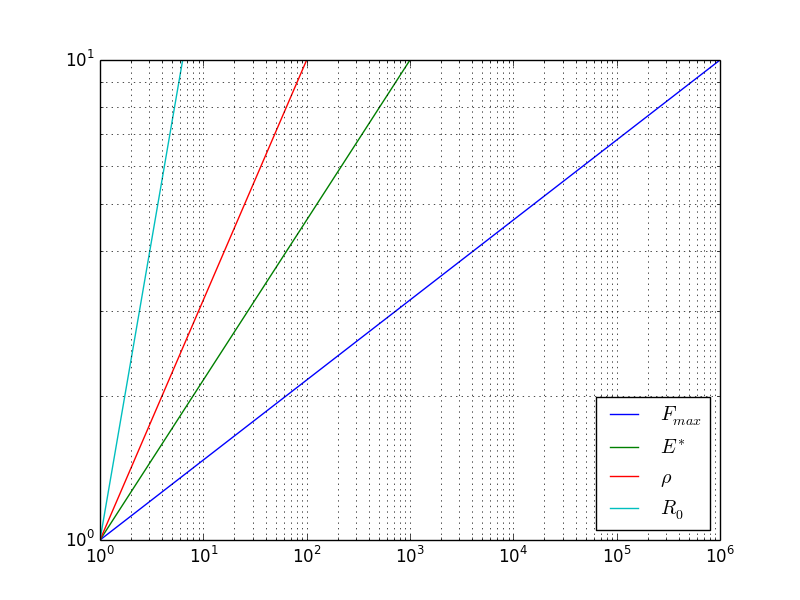
\includegraphics[width = 0.75 \textwidth]{chapters/figures/stability_curves}
% \caption{Curves showing the rate of response to timestep on the various normal-contact parameters.}\label{fig:stability-curves}
% \end{figure}

% It is apparent that simulations become less stable primarily as the pebble diameter decreases and then slightly less so for decreasing density and increasing the effective Young's modulus. It takes a rather large increase in the maximum contact force to cause the stable timestep to decrease. This is a fortunate result as it is primarily material properties which dictate stability of a DEM simulation. If external pressures increase and cause increases in the maximum normal contact force in the ensemble, it is unlikely to cause instabilities in the model. The result also provides insight into scaling of physical parameters to allow larger timesteps and thereby shorter overall duration of simulations.

The ceramic materials identified for breeders have relatively high Young's moduli, on the order of \si{10^{10} Pa}. The smallest radius will be on the order of \si{10^{-4} m}. The ceramic density is approximately on the scale of \si{10^{4} kg/m^3}. Finally, to prevent pebbles from cracking in the ensemble, it is reasonable to assume that the maximum contact forces will on the order of \si{10^2 N}. These values lead to a necessary timestep of

\begin{equation}
	\delta t_c \propto 10^{-7} \si{s}
\end{equation}

For a simulation that may last several hundreds of seconds of real time, this then requires more than 10$^9$ timesteps. If we have 10$^4$ particles in the simulation, each having their position integrated over a billion times, it becomes obvious that computational time is a major issue for our simulations of nuclear heating of ceramic breeder pebbles. If we are able to reduce the critical timestep (while perhaps decreasing the simulation time), the simulations will be much more practical for use.



\subsection{Simulation acceleration with scaled material properties}
I wish to rewrite Eq.~\ref{eq:rayleigh-timestep} to facilitate a discussion on the parameters. Isolating each material term gives, 

\begin{equation}
	\delta t_c \propto R_i \times \frac{\sqrt{2(1+\nu_i)}}{0.1631 \nu_i + 0.876605}  \times \rho_i^{1/2} \times E_i^{-1/2}
\end{equation}

[pretty sure the approximation for $\nu$ only works when it's less than 1 so can't scale. must find out for sure.]

The most direct effect would come from scaling the radius 





\section{Pebble failure modeling}
\label{failureDiscussion}
%In modeling pebble failure, there are two main tasks. The first is to develop a model for predicting a pebble failure event; { i.e.} what load (mechanical or thermal) will cause a pebble to crack, shatter, fracture, etc. The second is to develop a model which simulates the failure of that pebble; { i.e.} a scheme to treat a cracked, shattered, or crushed pebble in the assembly. 

The discrete element method has been used for studies in a variety of fields for studying inter-particle forces and the homogeneously distributed force networks that arise in packed beds (for example, see Ref.~\cite{Makse2000}). The discrete element method was also used in the fusion community to attempt to model failure initiation and propagation\cite{Annabattula2012a, Zhao2012, Zhao2013}. They too observed that a relatively few number of high-force networks, distributed troughought the bed supported the external mechanical loads. The even distribution of the force networks was used to defend the development of a probability-based predictor for failure. We make use of the probability argument of Zhao, {et al.} for the current study\cite{Zhao2013}. Their basic premise is that probability distributions of strength curves for pebble crushing have been observed (see, for example crush loads of Ref.~\cite{Tsuchiya1998}). Then in DEM models, a probability distribution of inter-particle forces are also observed. Overlaying the two probabilities resulted in seemingly random locations of pebbles satisfying the failure criteria -- not strictly along the high-force chains running through packed beds.

We apply the theory of Zhao, { et al.} in the following manner. If pebbles fail at random locations, we may de-couple the task of predicting pebble failure ({ i.e.} finding the mechanical or thermal load that causes a pebble to fail) from the task of modeling the ramifications of pebble failure. In our model, we begin with a starting point of a packed bed and then simply flag pebbles at random for `failing'. For our first model of failure, after a pebble has been flagged it is removed from the system entirely. The removal disrupts the meta-static state of the ensemble and the remaining pebbles re-settle. In reality, the ceramic pebbles generally break into just a few large pieces that remain in the system. Under development is a method for recreating that behavior in the DEM domain, it will be reported in future studies.

%Experiments on crushing single, brittle pebbles reveal that there are a number of failure modes\cite{Wu2004}. At one end, the pebble may simply crack and continue to hold a load for some time. At the other extreme, a pebble may crush virtually into a dust. We concern ourselves with the latter for this study. When a pebble in our simulation has been flagged for failure, we remove the pebble completely from the ensemble and then allow the remaining pebbles to rearrange to compensate for the lack of equilibrium on their contact forces. 


%\section{Simulation methods}
%\label{back} 
Our three-dimensional system consists of mono-dispersed particles of diameter $d$. The particles are constrained by two rigid walls in the $x$-direction at locations of $x = \pm 10d$  and periodic boundary conditions in the $y$-direction located at $y = \pm 7.5d$. Gravity acts in the downward $z$-direction and the particles are bound from below by a rigid wall at $z=0$. The size of the system allows approximately 10~000 particles to fill to a height of approximately $z = 30d$. The volume was chosen to represent the long, tall, narrow channels seen in many solid breeder module designs\cite{ Cho2008, Poitevin2010, Enoeda2003}.


\subsection{Material properties}
For this study, the material was chosen as lithium metatinatate with all properties coming from Ref.~\cite{Gierszewski1998}; they are summarized in Table~\ref{tab:matProps}

\begin {table}[tp] %
\caption{Maximum load and nominal tension.}
\label {tab:matProps} \centering %
\begin {tabular}{ cccccc }
\toprule %
E            &     $\nu$    &       k         &    C             &   $\alpha$                     \\
(GPa)    &                     &(W/m-K)  &  (J/kg-K)  &   (1/K)                                   \\\toprule
126       &      0.24       &  2.5          &  1156       &  $15\times10^{-6}$       \\\bottomrule
\end{tabular}
\end{table}



\subsection{Methodology}
\label{method}
\begin{figure}[t]
	\centering
	\begin{subfigure}[b]{0.23\textwidth}
		\centering
		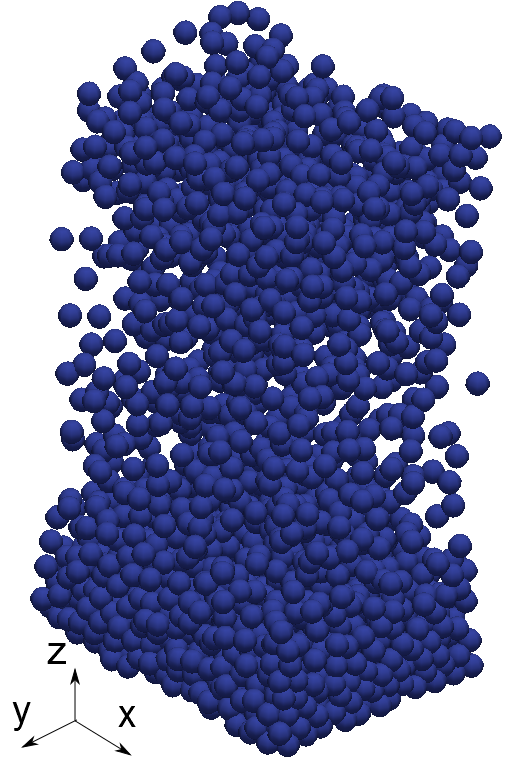
\includegraphics[width=\textwidth]{chapters/figures/fill01.png}
	\end{subfigure}
	%\begin{subfigure}[b]{0.15\textwidth}
	%	\centering
	%	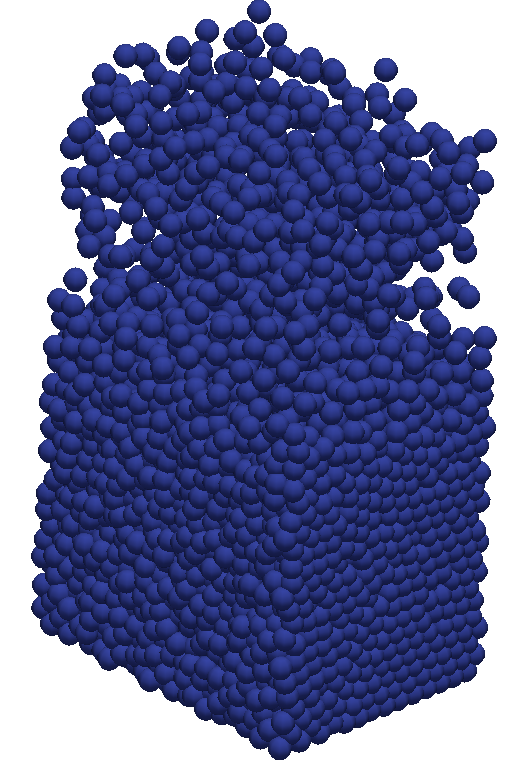
\includegraphics[width=\textwidth]{chapters/figures/fill02.png}
	%\end{subfigure}
	\begin{subfigure}[b]{0.23\textwidth}
		\centering
		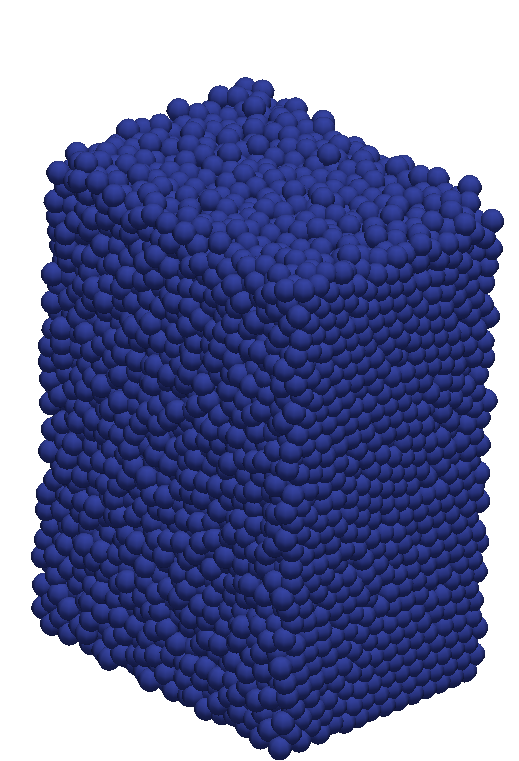
\includegraphics[width=\textwidth]{chapters/figures/fill03.png}
	\end{subfigure}
	\caption{Demonstrating the pouring process of $N = 10~550$ pebbles into the control volume with an early (left) and late (right) snapshot.}
\label{fig:fill01}
\end{figure}

\begin{figure}[t]
	\centering
	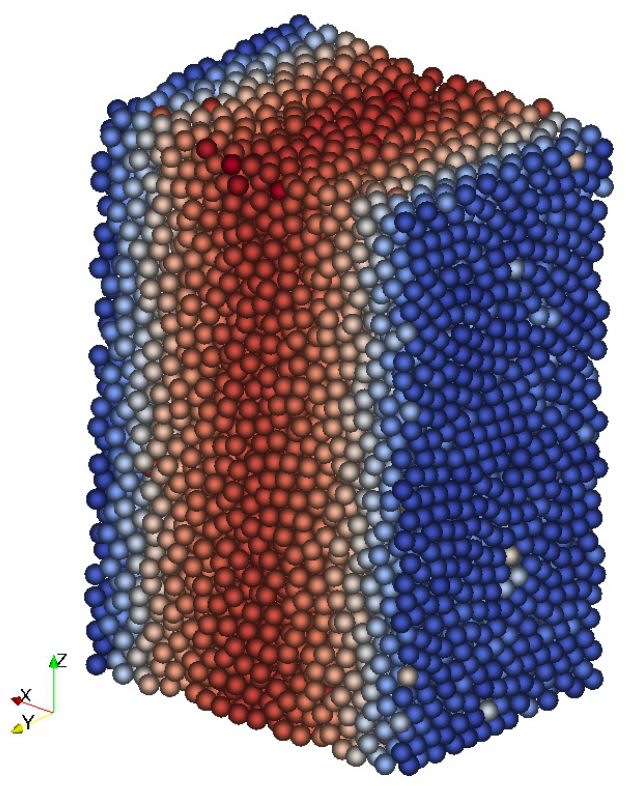
\includegraphics[trim=1cm 8cm 3cm 4cm, width=0.4\textwidth]{chapters/figures/pebbleBedTemperature}
	\caption{Temperature distribution of pebbles in the $10\%$ failed bed. At the end of steady-state heating, a one-dimensional profile is evident in all pebble beds studied here. The pebbles are receiving nuclear heating. Cooling proceeds through the pebbles in contact with the walls in the $x$-direction. [color online]}
\label{fig:pebbleBedTemperature}
\end{figure}


All the test cases begin with a common starting point of a filled, lightly packed volume of 10~550 pebbles. The pebbles are poured into the volume from above and come to rest under the influence of gravity (see Fig.~\ref{fig:fill01}). Initially, to recreate how we may pack solid breeders in reality, we attempted vibration simulations in order to pack the pebbles into a more dense state. However, we found the same packing states (from a void fraction standpoint) could be realized in a more computationally-simple manner by lowering a $z$-plane wall onto the top of the packed bed until it experienced some small force. This pour-press-packing routine was repeated many times and all the beds exhibited the same force on the top wall at roughly the same packing fraction. We took the last case, with a packing fraction (volume of $N$ pebbles per total volume) of $\phi_\text{bl}= 62.9\%$, as our baseline configuration. The packed bed state was saved and used as a starting point for numerous `failed' cases to be described later.

For the baseline case, we assigned an initial temperature of $T_\text{ref}$ to both the pebbles and the $x$ walls, then set a constant nuclear heating source on each pebble. The nuclear energy raised the temperature of the pebbles while the walls remained at $T_\text{ref}$ for cooling. The process ran until a steady state was reached (for example, see Fig.~\ref{fig:pebbleBedTemperature}); the total thermal energy of the bed, $E =\sum_i^N m_iC_i T_i$, was monitored and the simulation completed when the value was constant. At steady state, we analyzed thermomechanical characteristics of the pebble bed such as effective thermal conductivity, average coordination number, temperature profiles in the bed, and inter-particle contact forces.

As mentioned in Sec.~\ref{failureDiscussion}, in this study we model pebble failure without considering the cause of failure. This is done by randomly selecting pebbles from the ensemble, regardless of forces acting upon the pebble, and removing them entirely. When a pebble is removed, the neighboring pebbles react due to the imbalance of forces and the bed settles into a new configuration. We differentiated the failed beds by their percentage of failed pebbles: $\eta = $ number of failed pebbles per original ensemble size. After failing we again applied our heating routine.
\section{DEM solver}\label{sec:dem-solver}

Time-discretization of the integration of Eq.~\ref{eq:newtons-first} is handled by the core Large-scale Atomic/Molecular Massively Parallel Simulator (LAMMPS) code released by Sandia National Laboratories\cite{Plimpton1995, Parks2008}. The code calculates velocity and position via the semi-explicit velocity-Verlet integration. The algorithm is stable with a global error of approximately $O(\Delta t^2)$ for displacement; details can be found in Ref.~\cite{Grubmuller1991}.

In the process of the study, to demonstrate the ability of the dynamic integration to capture resettling (and any possibly asymmetries), some beds were generated wherein the failure of pebbles was slightly localized near one or both $x$-walls. The profile of the pebbles near the top of the stack, after resettling, are shown in Fig.~\ref{fig:settlingStudy}. 

In our work, we occasionally required a fully quiesced bed. To determine when this occurred, the total kinetic energy of the entire ensemble was monitored and a packed bed was considered to have completely settled once the kinetic energy of the system was less than $10^{-9}$; similar to the process described in Ref.~\cite{Silbert2002a}. 


The granular heat transfer equations (Eqs.~\ref{conductance}-\ref{thermoFirstLaw}) are layered onto the LAMMPS code via a package of code named LIGGGHTS (LAMMPS Improved for General Granular and Granular Heat Transfer Simulations \cite{kloss2012a}). Parallelization of the code is straightforward with LAMMPS and we run the code on 128 nodes of UCLA's Hoffman2 cluster for typical run times of 18 to 24 hours per routine ({e.g.} filling, packing, heating, etc.).

\section{Results and discussions}
\label{results}

\begin{figure}[t]
	\centering
	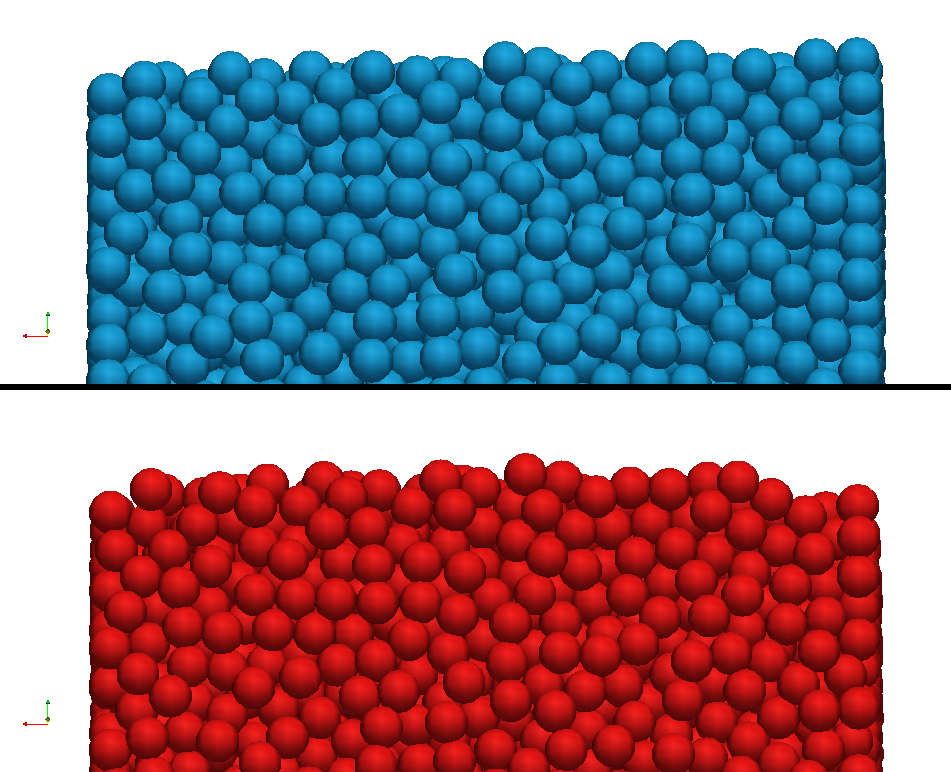
\includegraphics[width=0.4\textwidth]{chapters/figures/settlingStudy}
	\caption{Demonstrating the dynamic resettling from an example study done on location bias to pebble failure. The top image had the pebbles near the left wall biased to fail. The bottom image had a bias for the pebbles near both walls to fail. The lines are drawn as an aid to the eye.}
\label{fig:settlingStudy}
\end{figure}


The aim of this study was both to discover the impact of pebble failure on thermomechanical properties as well as determine the impact as a function of the number of failed pebbles. To satisfy the latter, we created beds with $\eta = 1\%$, $5\%$, $10\%$, and $15\%$ of pebbles failed. 

We first compare steady-state temperature profiles in the test beds against the one-dimensional theory of Eq.\ref{heateqn}. To find the temperature profile in $x$, we create volumes of width $\Delta x$ that extend through the limits of the $y$- and $z$-directions. We then find the $n$ pebbles residing in the slices and take the mean value of their temperatures, $\langle T\rangle = \sum_{i}^n T_i / n$ of all pebble temperatures that have coordinates inside the slice. Below we will omit the notation $\langle T \rangle$ with the understanding that temperatures are volume-averages. Using the volume slices, we also find the average coordination number, $\langle Z \rangle = \sum_{i}^n Z_i / n$, normalized average contact force, $\langle F^* \rangle=\left[\langle F \rangle/\langle F_{bl} \rangle_\text{max}\right]^{1/3}$, and the normalized average temperature difference between pebbles in the slice, $\langle \Delta T_{ij} \rangle / (T_0 - T_s)_\text{bl}$; parameters which are discussed later.

When analytically solving Eq.~\ref{thermoFirstLaw}, we introduce non-dimensional temperature, $\theta_\text{1D} = (T -T_s)/(T_0-T_s)$, and spatial, $x^* = x/L$, variables and the solution becomes purely geometric; $\theta_\text{1D} = 1-x^{*2}$. We plot this theoretical solution against the temperature profiles coming from the steady-state DEM simulation in Fig.~\ref{fig:tempProfile}. We find that all our models had a nearly perfect match to a one-dimensional prediction, validating the calculation of effective thermal conductivity in this study. 

Another concern we had for pebble failure, was the phenomenon of `jamming' during resettling that would possibly leave pebbles isolated from their neighbors (apart from those they are resting upon). Such an isolated pebble would have no strong pathway for heat transfer and heat up much higher than that of its neighbors. Evidence of pebble isolation and `hot-spots' would be apparent in Fig.~\ref{fig:tempProfile} as localized deviations of data points from the quadratic profile. However, no deviations are seen in the data and we conclude that hot-spots will not be a concern in a packed bed.

\begin{figure}[t]
	\centering
	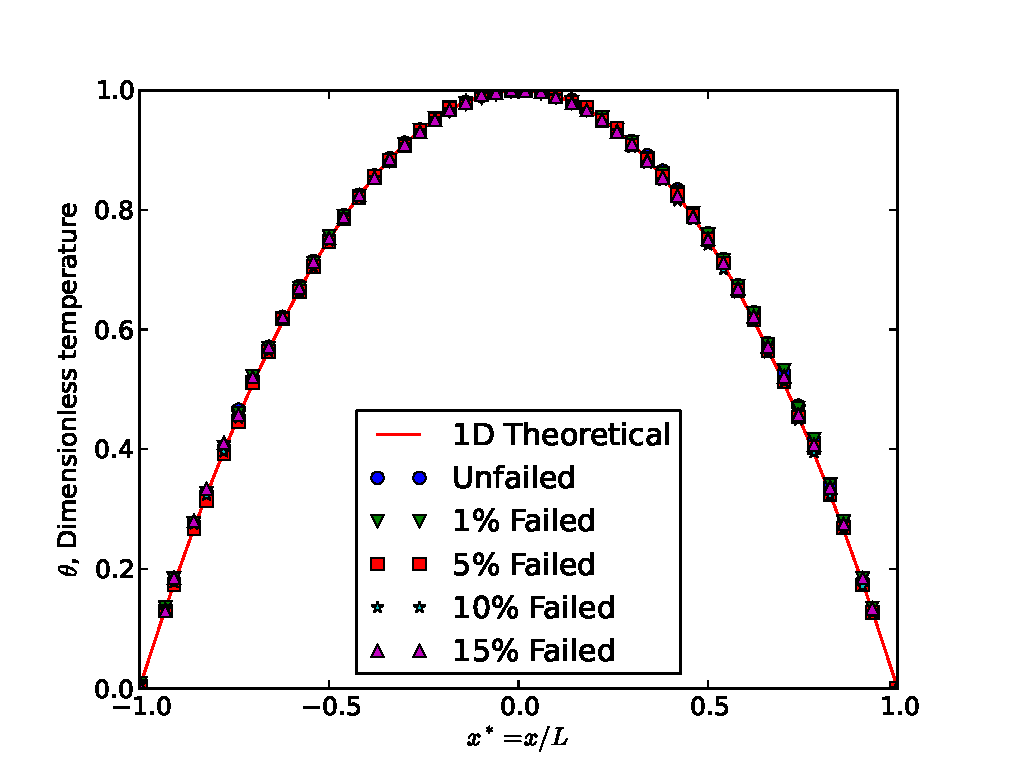
\includegraphics[width=0.5\textwidth]{chapters/figures/tempProfiles}
	\caption{The non-dimensional temperature profiles for each test case follow the theoretical shape of a one-dimensional, constant $k$, continuum solution.}
\label{fig:tempProfile}
\end{figure}



\begin{figure}[t]
	\centering
	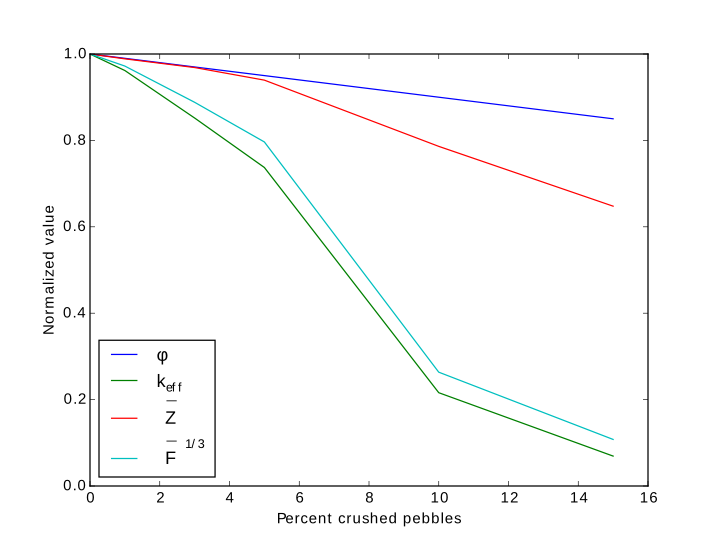
\includegraphics[width=0.5\textwidth]{chapters/figures/kEff_packingFraction}
	\caption{The normalized effective thermal conductivity (solid line) follows an exponential decay relationship with amount of failed pebbles. The normalized packing fraction (dashed line), compared to thermal conductivity, is relatively constant and is more closely fit to a linear reduction.}
\label{fig:packingFraction}
\end{figure}

\begin{figure}[t]
	\centering
	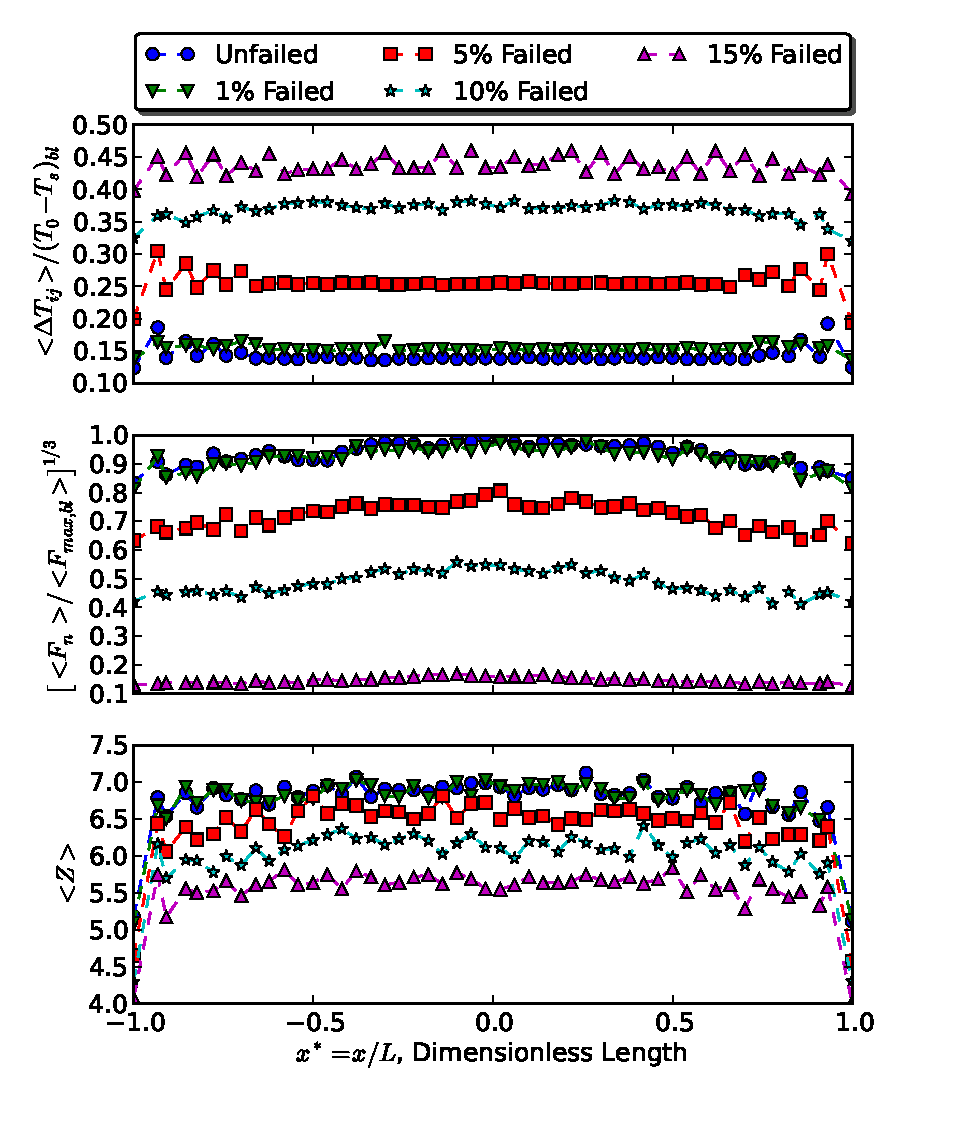
\includegraphics[width=0.5\textwidth]{chapters/figures/z_f_deltaT_subPlots}
	\caption{Average temperature differences between neighboring pebbles (top), contact forces (middle) and coordination numbers (bottom). The profiles of average coordination number and contact forces in the bed decrease in value with increasing pebble failure. Fewer and weaker contacts will reduce the possible paths of heat transfer from a pebble and this results in higher average temperatures between neighbors.}
\label{fig:coordProfiles}
\end{figure}


The effective thermal conductivity is found for all of our pebble beds, via Eq.~\ref{eq:etc}, then normalized against the conductivity of the baseline ensemble ($k_\text{eff}^* = k_\text{failed}/k_\text{bl}$). Figure~\ref{fig:packingFraction} shows the decreasing ETC with pebble failure. When $15\%$ of the pebbles are crushed in a pebble bed, the ETC has fallen all the way to only $k_\text{eff}^*=0.30$. This large reduction is especially important in light of the already poor thermal management of virgin pebble beds that, even in helium environments, have been experimentally measured at only approximately 1~W/m-K (see, { e.g.}, Refs.~\cite{Reimann2002, Piazza2002}). In well-packed pebble beds, the ETC is generally related to the packing fraction. In Fig.~\ref{fig:packingFraction}, this relationship seems weak as the effective conductivity drops much more rapidly than does the packing fraction as the number of broken pebbles in the ensemble increases. To find the cause of decrease in conductivity and to make use of the information provided by DEM tools, we look to other parameters than the packing fraction.

From Eq.~\ref{thermoFirstLaw}, in the steady-state, the energy input by nuclear heating must be balanced by the transport of heat out of a pebble into its neighbors. Inter-particle heat transfer is dictated by the number of neighboring contacts, temperature difference between pebbles, and the thermal conductance, $h_{ij}$ through the contact area. The thermal conductance is, itself, a function of material properties  (which are essentially constant here) and the force at the contact, going as $h_{ij} \propto F_n^{1/3}$. Thus, the net heat out is a function of the three variables as
\begin{align}
Q_\text{net} =f( Z, F_n^{1/3}, \Delta T)
\end{align}



The variables affecting $Q_\text{net}$ are plotted in Fig.~\ref{fig:coordProfiles}. The average coordination number, shown in the bottom plot, decreases from a mid-line value of about 7.0 at the steady-state of the baseline case down to a mid-line value of 5.5 for the 15\% failed bed; a reduction of about 80\%. But this number doesn't compare with the large reduction in ETC which was $k_\text{eff}^*=0.30$. Clearly, there are fewer contacts in the pebble bed after failure but this alone does not account for the reduction in ETC.

Much more dramatic, seen in the center plot, is the reduction in average normal force seen by pebbles after many of the neighbors fail and are removed from the system. From the baseline down to the 15\% failed case, the contact forces are dramatically reduced to about $\langle F^* \rangle=0.1$.This reduction in force is joined by an increase in average neighbor temperatures which are 3 times higher for the bed with most failed pebbles when compared to the baseline. 

The results shown in Fig.~\ref{fig:coordProfiles} demonstrate that the heat transfer through a pebble bed is simultaneously a function of the coordination number and inter-particle contact forces -- which are both reduced as pebbles in the bed fail -- as well as the temperature difference between pebbles at steady state -- which increases as pebbles in the ensemble fail. Interestingly, when a pebble bed has lower overall inter-particle contact forces fewer particles would be expected to break. This would imply that pebble breakage is self-dampening; as pebbles begin to break the ensemble quickly relaxes and avoids future pebble failure. So while we induced failure up to $\eta = 15\%$, such large values may not occur in real beds. 

Another feature of Fig.~\ref{fig:coordProfiles} worth noting is the increase in averaged normal contact forces near the center of the bed relative to the walls. In the assumptions used to develop this simulation, we had noted the lack of localized force concentrations in a bed under an external mechanical load. However, in these results, owing to the nuclear heating temperature profile and thermal expansion of each pebble, there is a bias toward higher forces in the center of the bed. This result highlights the need for a model to predict failure initiation in place of the assumption of random pebble failure. 
%There are dramatic decreases near the walls for two reasons. The first being that contact of a pebble with a wall is not counted in the overall coordination number. The second is the forced ordering that pebbles experience near walls that is absent from the random packing in the bulk. Away from the walls, there is a clear decreasing trend in the coordination number as the pebble failure increases. From Eq.~\ref{thermoFirstLaw}, the heat transfer from a pebble is a function of the number of neighbors with which the pebble is in contact. 



\section{Conclusions}
\label{concs}
The current study aimed at properly simulating a pebble bed with a specified fraction of the pebbles failing during operation; then determining the repercussions of the failures as they affect the macroscopic property of effective thermal conductivity. We used the assumption of homogeneous, random locations of pebble failure to induce a failure routine without requiring external loads on the bed to permit beds that could be directly compared. After heating to a steady-state, an effective thermal conductivity was calculated for the pebble bed. The results show that small amounts of pebble failure correspond to large decreases in the conductive transport of energy through the pebble bed. The increase was due primarily to a drop in the inter-particle forces which lead to a large increase in temperature differences between neighboring pebbles. We note again, however, that this value has been calculated in the absence of interstitial gas so the results apply only to the reduction in energy transferred via inter-particle conduction.


The assumption of homogeneous distribution of pebble failure was found to be inappropriate after a pebble bed reached steady state nuclear heating. The scheme assumes no localization of average forces in the bed but we found an average force profile that had a maximum at the center and minimum at the walls. The next step of modeling will eliminate the error of such an assumption as we must combine failure prediction to failure outcome modeling. 





